\chapter{Receiver calibration}\label{chap:calibration}

% **************************** Define Graphics Path **************************
\ifpdf
    \graphicspath{{calibration/figs/Raster/}{calibration/figs/PDF/}{calibration/figs/}}
\else
    \graphicspath{{calibration/figs/Vector/}{calibration/figs/}}
\fi


With a working instrument capable of taking measurements in the field, the next step towards detection of the 21-cm signature is calibration of the experimental apparatus. There are many forms of calibration from physical antenna or ground plane modifications to numerical post-processing methods such as correctional atmospheric modelling. The need for more accurate cosmic signal measurements against the cacophony of unwanted noise demands finer degrees of calibration through the development of novel methods. At the current technological aim of millikelvin-level calibration, minute differences in an instrument’s electrical properties can skew spectral measurements enough to hamper a cosmological detection. In the previous chapter, we detailed the system architecture designed to minimise these distortions. Here we present a procedure to calibrate out the remaining systematic effects. The task has encompassed decades of research starting in the 1950’s where \citet{bauer_rothe} and \citet{rothe_dahlke} introduced a wave formulation of noise to microwave systems\footnote{\citet{bauer_rothe} presented in English by \citet{penfield}.} before a mathematical prescription to eliminate these noise waves through the derivation of “noise wave parameters” was conceived by \citet{meys} in 1978. This method, which inspires many contemporary radiometric calibration procedures, relies on the relative differences between sequential measurements of known passive devices to divide out small-timescale variability through a method known as “Dicke switching”, named after famed astronomer Robert Dicke. This relative calibration was utilised into the late 2000’s when \citet{edges_limits} placed a lower limit on the duration of the reionisation epoch at $\Delta z < 0.06$.

It was quickly understood that the extraction of further information from 21-cm experimentation required a more powerful calibration method and work commenced to reformulate the noise wave parameters under an “absolute” calibration procedure which offered a more comprehensive derivation by referencing all measurements to an absolute temperature scale as well as expanding compatibility with instruments of increasing bandwidth \citep{rogersCal}. It was this absolute calibration that was used in the 2018 EDGES measurement where the authors quote a 20 mK calibration accuracy \citep{edgesNature, edgesCal}. In response to the controversy surrounding the EDGES experiment, we have strived to improve the methodology and address discrepancies in the procedure through the introduction of a Bayesian calibration framework which we formulate over the following sections.


% =========================================
\section{Calibration formalism}\label{sec:formalism}
The noise necessitating calibration arises during measurements. For a global experiment such as REACH, we measure a sky temperature $\T{sky}(\Omega, \nu, t)$ as a function of the direction $\Omega$, frequency $\nu$ and time $t$ which can be broken down into two primary components: the global 21-cm signal $T_{21}$ and astrophysical foregrounds $\T{f}$
\begin{equation}
    \label{tsky}
    \T{sky}(\Omega, \nu, t) = T_{21}(\nu) + \T{f}(\Omega, \nu, t).
\end{equation}
Sky signals absorbed by the antenna convolve with the normalised antenna directivity $B$ ,introducing systematic noise represented by our random noise term $N_{\mathrm{data}}$.
\begin{equation}\label{eqn:bayestsource}
    D(\nu, t) = \int \T{sky}(\Omega, \nu, t) B(\Omega, \nu)\mathrm{d}\Omega + N_{\mathrm{data}}.
\end{equation}
Thus, our 21-cm signature can be formulated as
\begin{equation}\label{signal}
  T_{21} \approx D(\nu, t) - \int\T{f}(\Omega, \nu, t)B(\Omega, \nu)\mathrm{d}\Omega - N_{\mathrm{data}}.
\end{equation}
A diagram illustrating the evolution of the sky signal during this process in shown in \cref{fig:nsfig}.
\begin{figure}
    \centering
    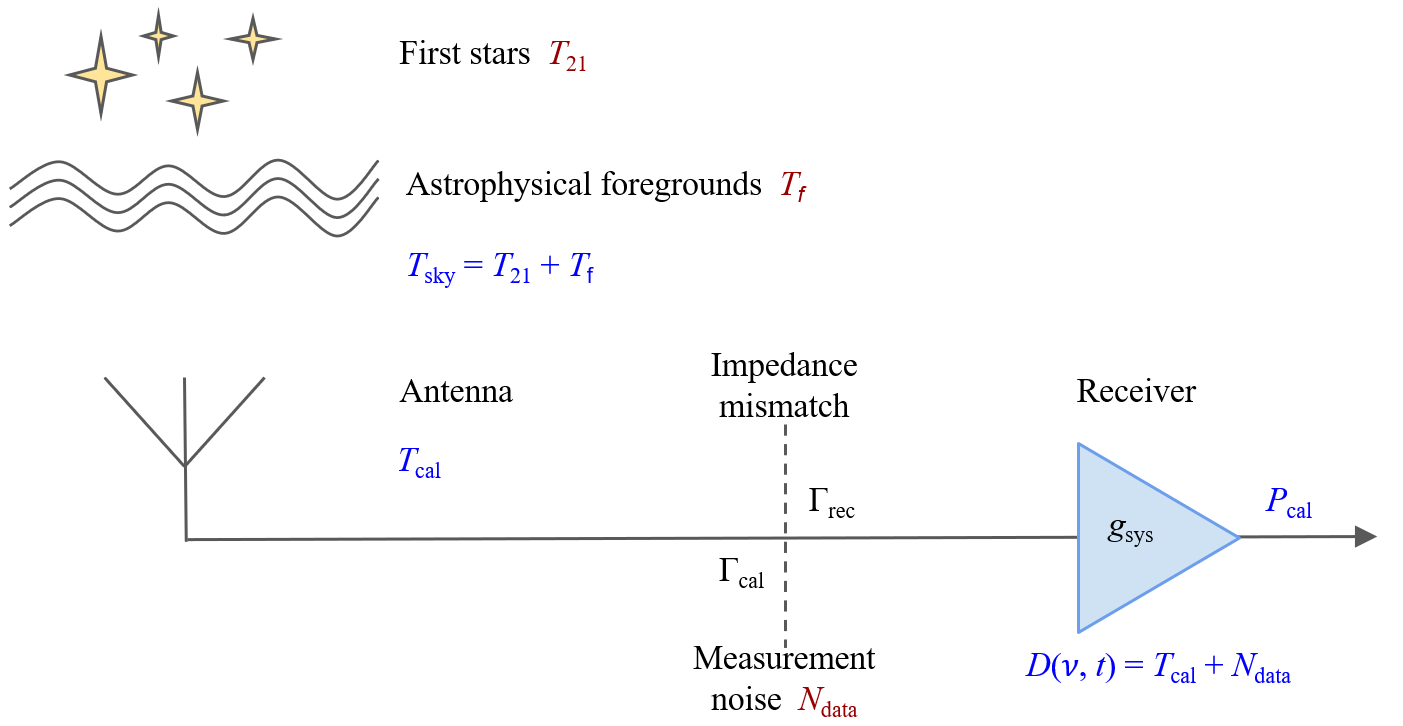
\includegraphics[width=.7\textwidth]{nsdiag}
    \caption{Diagram showing the evolution of the 21-cm signal hampered by astrophysical foregrounds, convolvution with the antenna beam and the emergence of measurement noise before calibration to retrieve the sky temperature.}
    \label{fig:nsfig}
\end{figure}
The integral in \cref{signal} is assessed through foreground and beam modelling techniques such as those discussed in \citet{dom} while modelling of $N_{\mathrm{data}}$ from the (statistical) properties of $D(\nu, t)$ is accomplished through calibration.

The standard calibration strategy follows the method introduced by Dicke to characterise systematic features in radio-frequency instruments \citep{dickeplus} and is widely used in experiments such as EDGES \citep{edgesCal} and LOFAR \citep{lofarCal} to evaluate the spectral index of the sky's diffuse radio background \citep{rogersCal}. The technique involves measurements of two internal reference standards; a load and a noise source, in addition to a series of external calibration sources attached to the receiver input in lieu of the antenna. Historically these include an ambient-temperature ‘cold’ load, a ‘hot’ load heated to $\sim 400$ K, an open-ended cable and a shorted cable as detailed previously in \cref{fig:dicke}.

During a calibration measurement, power spectral densities (PSDs) are taken of each Dicke switch position; the receiver input ($\psd{cal}$), the internal reference load ($\psd{L}$) and the internal reference noise source ($\psd{NS}$) \citep{edgesCal}. These measurements are used to calculate a preliminary `uncalibrated' antenna temperature $\T{cal}^*$
\begin{equation}
  \label{eqn:tantstar}
  \T{cal}^* = \T{NS} \left(\frac{\psd{cal}-\psd{L}}{\psd{NS}-\psd{L}}\right) + \T{L},
\end{equation}
where $\T{L}$ and $\T{NS}$ are assumptions for the noise temperature of the internal reference load and excess noise temperature of the internal noise source above ambient, respectively. This comparison of sequential power measurements serves as the `relative' calibration which removes time-dependent variations in system gain emerging from individual components or technical capabilities of the instrument \citep{edgesCal}. These PSD measurements can be expanded in terms of specific response contributions with the input power spectra being
\begin{multline}
  \label{eqn:pant}
  \psd{cal} = g_{\mathrm{sys}} \Bigg[ \T{cal}\left(1-|\Ga|^2\right)\left|\frac{\sqrt{1 - |\G{rec}|^2}}{1-\Ga\G{rec}}\right|^2 + \T{unc}|\Ga|^2\left|\frac{\sqrt{1 - |\G{rec}|^2}}{1-\Ga\G{rec}}\right|^2 \\
  + \T{cos}\operatorname{Re}\left(\Ga\frac{\sqrt{1 - |\G{rec}|^2}}{1-\Ga\G{rec}}\right) + \T{sin}\operatorname{Im}\left(\Ga\frac{\sqrt{1 - |\G{rec}|^2}}{1-\Ga\G{rec}}\right) 
  + T_0 \Bigg],
\end{multline}
where $\Ga$ and $\G{rec}$ are the measured reflection coefficients of the device connected to the receiver input and receiver itself respectively. $g_{\mathrm{sys}}$ is the system gain referenced to the receiver input and $\T{cal}$ is our calibrated input temperature. $\T{unc}$, $\T{cos}$, and $\T{sin}$ are the ‘noise wave parameters’ introduced by \citet{meys} to calibrate the instrument \footnote{equivalent to $\T{a}$ $\T{b}$, and $\T{c}$ in his notation}. $\T{unc}$ represents the portion of noise reflected by the antenna that is uncorrelated with the output noise of the LNA while $\T{cos}$ and $\T{sin}$ represent the portions correlated with LNA noise \citep{edgesCal, rogersCal}. The phase in which these reflected noise waves re-enter the receiver is described by the Re() and Im() arguments of \cref{eqn:pant}\footnote{These arguments are equivalent to the $\alpha$ term in the EDGES notation \cite{edgesCal} and analogous to $\phi$ in the Meys formulation \citep{meys}}. In the EDGES experiment, the noise wave parameter quantities are modelled using seven-term polynomials in frequency.

The PSDs for the internal reference load and noise source can similarly be expressed as in \cref{eqn:pant}. However, since the reflection coefficients of the internal references are assumed to be small, we approximate them as zeros in order to simplify the equations
\begin{equation}
  \label{eqn:pl}
  \psd{L} = g_{\mathrm{sys}}^*[\T{L}\left(1-|\G{rec}|^2\right)+T_{0}^*],
\end{equation}
\begin{equation}
  \label{eqn:pns}
  \psd{NS} = g_{\mathrm{sys}}^*[\left(\T{L}+\T{NS}\right)\left(1-|\G{rec}|^2\right)+T_{0}^*].
\end{equation}
As shown in \cref{fig:dicke}, the internal references may be on a separate reference plane than the receiver input, resulting in a system gain $g_{\mathrm{sys}}^*$ and a noise offset $T_{0}^*$ different from those defined in \cref{eqn:pant}. This effect is taken into account by two additional scale and offset parameters, $C_1$ and $C_2$, introduced by EDGES \citep{edgesCal}.

Since $C_1$ and $C_2$ also correct for first-order assumptions in the noise temperatures of the internal reference load and noise source, we have chosen to absorb these terms into $\T{L}$ and $\T{NS}$ in our analysis. This adjustment allows all calibration parameters, $\T{unc}$, $\T{cos}$, $\T{sin}$, and the ‘effective’ $\T{NS}$ and $\T{L}$, to be solved for in units of kelvin, facilitating a joint solution of parameters. Expanding \cref{eqn:tantstar} using \cref{eqn:pant,eqn:pl,eqn:pns} yields a linear identity providing a relationship between the uncalibrated input temperature and a final calibrated temperature of any device connected to the receiver input
\begin{multline}
  \label{eqn:caleqn}
  \T{NS}\left( \frac{\psd{cal} - \psd{L}}{\psd{NS} - \psd{L}} \right) + \T{L} = \T{cal}\left[ \frac{1-|\Ga|^2}{|1-\Ga\G{rec}|^2} \right]
  + \T{unc}\left[ \frac{|\Ga|^2}{|1-\Ga\G{rec}|^2} \right] \\
  + \T{cos}\left[ \frac{\operatorname{Re}\left(\frac{\Ga}{1-\Ga\G{rec}}\right)}{\sqrt{1-|\G{rec}|^2}} \right]
  + \T{sin}\left[ \frac{\operatorname{Im}\left(\frac{\Ga}{1-\Ga\G{rec}}\right)}{\sqrt{1-|\G{rec}|^2}} \right],
\end{multline}
where all parameters are frequency-dependent though not explicitly shown for simplicity of notation. During a calibration procedure, $\T{cal}$, $\Ga$ and $\G{rec}$ are measured along with the PSDs while $g_{\mathrm{sys}}$ and $\T{0}$ are calibrated out via the `relative' calibration procedure inherent to \cref{eqn:tantstar}. As stated in \cref{sec:frontend}, the $50 \Omega$ cold and hot loads exhibit the main temperature references needed for $\T{L}$ and $\T{NS}$ while delayed reflection in the calibration cables allow for the derivation of $\T{unc}$, $\T{cos}$ and $\T{sin}$ by simulating an antenna observing an ambient temperature sky \citep{rogersCal}.


% =========================================
\section{Bayesian parameter derivation}\label{sec:bayes}
From an instrumentation perspective, a possible source of the systematics thought to blemish the EDGES measurement is the calibration of their instrument in a controlled laboratory setting separate from the environment in which astrophysical observations take place. At the milli-kelvin level, these environmental effects may be non trivial. Parameters related to the physical instrument are expected to change such as the antenna response due to heat expansion or impedance fluctuations of delicate front-end components. As corroborated by the various experiments in the REFER TO RESULTS SECTION, this may especially be the case with regards to how the calibration parameters change between observation runs. Furthermore, the fixed seven-term polynomial used by EDGES to model all of their noise wave parameters may underfit or overfit individual parameters and thus `fit out' data useful for determining systematics or potentially even the 21-cm signal itself if a joint fit is performed.

In response to these concerns, we have developed a calibration pipeline that improves on the strategies presented in \citet{edgesCal} and introduce a novel Bayesian methodology using conjugate priors, allowing for a dynamic application of our algorithm in the field with astrophysical data collection regardless of system complexity. Also included are model selection procedures for the optimisation of  individual noise wave parameters to combat overfitting and underfitting, the results of which converge with that of a least-squares approach when wide priors are adopted. Our pipeline easily incorporates many more calibration sources than the standard four as shown in \cref{sec:frontend} for increased constraints on noise wave parameters while identifying possible correlations between parameters. A schematic overview of our improved Bayesian calibration method is shown in \cref{fig:cal_flowchart}.
\begin{figure}
    \centering
    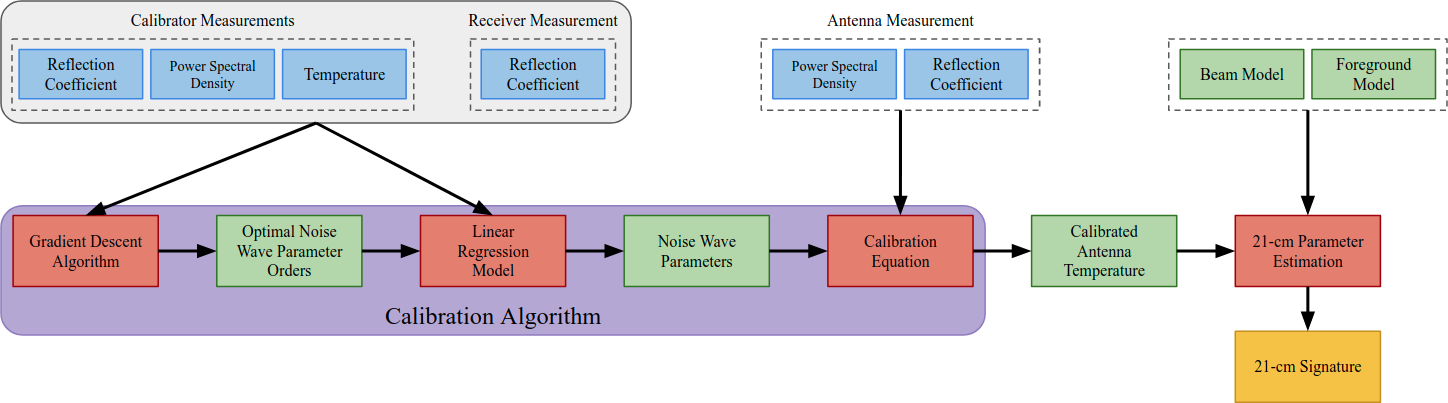
\includegraphics[width=\textwidth]{cal_flowchart}
    \caption{Outline of our Bayesian calibration algorithm. Blue blocks represent data to be taken, red blocks represent calculations and green blocks represent calculation outputs.}
    \label{fig:cal_flowchart}
\end{figure}

We first, simplify the notation of our approach by defining the following terms
\begin{equation}
  X_{\mathrm{unc}} = -\frac{|\Ga|^2}{ 1-|\Ga|^2}, 
\end{equation}
\begin{equation}\label{eqn:xl}
  X_{\mathrm{L}} = \frac{|1-\Ga\Gr|^2}{1-|\Ga|^2},
\end{equation}
\begin{equation}
  X_{\mathrm{cos}} = -\operatorname{Re}\left(\frac{\Ga}{1-\Ga\Gr} \times \frac{X_{\mathrm{L}}}{\sqrt{1-|\Gr|^2}}\right),
\end{equation}
\begin{equation}
  X_{\mathrm{sin}} = -\operatorname{Im}\left(\frac{\Ga}{1-\Ga\Gr} \times \frac{X_{\mathrm{L}}}{\sqrt{1-|\Gr|^2}}\right),
\end{equation}
\begin{equation}\label{eqn:xns}
  X_{\mathrm{NS}} = \left( \frac{P_{\mathrm{cal}}-P_{\mathrm{L}}}{P_{\mathrm{NS}}-P_{\mathrm{L}}} \right) X_{\mathrm{L}},
\end{equation}
which represent initial calibration measurements on $D$ in the frequency domain for the characterisation of $N_{\mathrm{data}}$ from \cref{eqn:bayestsource} via our noise wave parameters. Here we assume that calibration-related deviations of $D$ in the time domain are sufficiently curtailed through practical strategies such as temperature control of the receiver environment. Incorporating these equations into \cref{eqn:caleqn}, with some rearrangement, then gives
\begin{equation}
  X_{\mathrm{unc}}\T{unc} + X_{\mathrm{cos}}\T{cos} + X_{\mathrm{sin}}\T{sin} + X_{\mathrm{NS}}\T{NS} + X_{\mathrm{L}}\T{L} = \T{cal},
\end{equation}
at each frequency. We can see here that there are no squared or higher-order terms, allowing us to take advantage of the linear form by grouping the data and noise wave parameters into separate matrices
\begin{equation} \label{eqn:theta}
    \begin{split}
    \mathbfss{X} &\equiv \begin{pmatrix} 
        X_\mathrm{unc} \quad 
        X_\mathrm{cos} \quad
        X_\mathrm{sin} \quad
        X_\mathrm{NS} \quad
        X_\mathrm{L} \end{pmatrix}, \\
    \boldsymbol{\Theta} &\equiv \begin{pmatrix} 
        T_\mathrm{unc}\quad
        T_\mathrm{cos}\quad
        T_\mathrm{sin}\quad
        T_\mathrm{NS}\quad
        T_\mathrm{L}\end{pmatrix}^\top.
    \end{split}
\end{equation}

Under this formulation, all of our data; the reflection coefficient measurements and power spectral densities, are grouped in an $\mathbfss{X}$ vector which forms a matrix where one of the axes is frequency. The calibration parameters as frequency-dependent polynomials of varying degree are collected into a $\boldsymbol{\boldsymbol{\Theta}}$ vector which serves as our model describing $N_{\mathrm{data}}$. Applying these definitions condenses the calibration equation into
\begin{equation}\label{eqn:linearmodel}
  \y = \mathbfss{X}\boldsymbol{\boldsymbol{\Theta}}+\sigma,
\end{equation}
where $\y$ is a vector over frequency and $\sigma$ is a noise vector representing our error. Since EDGES assumes that each power spectral density measurement is frequency independent, we have assumed that $\sigma$ is a multivariate normal distribution. This assumption is implicit in the EDGES analysis in which they use a least-squares minimisation approach for solving model parameters.

For calibration of the receiver, we are concerned with the construction of predictive models of the noise wave parameters, $\boldsymbol{\Theta}$, in the context of some dataset, $\mathbfit{T}$. We can use $\boldsymbol{\Theta}$ to calculate the probability of observing the data given a specific set of noise wave parameters:
\begin{equation}\label{likelihood}
    p\big(\mathbfit{T} \given[\big] \boldsymbol{\Theta}, \sigma^2\big) = \frac{1}{2\pi \sigma^2}^{N/2}\exp{ \Bigg\{ -\frac{1}{2\sigma^2}\left(\mathbfit{T}-\mathbfss{X}\boldsymbol{\Theta}\right)^{\top}\left(\mathbfit{T} -\mathbfss{X}\boldsymbol{\Theta}\right) \Bigg\}},
\end{equation}
where, $N$ is the number of measurements. This distribution on the data is the \textit{likelihood}. For the purposes of calibration, $\mathbfit{T}$ may be $\y$ measurements or alternatively, $\mathbfit{T}_{\mathrm{sky}}$ for prediction of a sky signal. Our model must also specify a \textit{prior} distribution, quantifying our initial assumptions on the values and spread of our noise wave parameters which we specify as a multivariate normal inverse gamma distribution:
\begin{equation}
  \label{eqn:prior}
  p\left(\boldsymbol{\Theta}, \sigma^2\right) \propto \left(\frac{1}{\sigma^2}\right)^{a+1+\left(d/2\right)} \times \exp \left[ -\frac{1}{\sigma^2}\{b+\frac{1}{2}\left(\boldsymbol{\Theta}-\boldsymbol{\mu}_{\boldsymbol{\Theta}}\right)^{\top}\mathbfss{V}_{\boldsymbol{\Theta}}^{-1}\left(\boldsymbol{\Theta}-\boldsymbol{\mu}_{\boldsymbol{\Theta}}\right)\} \right],
\end{equation}
which is proportional up to an integration constant. Here, $a$ and $b$, which are greater than zero, along with $\mathbfss{V}_{\boldsymbol{\Theta}}$ and $\boldsymbol{\mu}_{\boldsymbol{\Theta}}$ represent our prior knowledge on the noise wave parameters. $d$ is the length of our vector $\boldsymbol{\Theta}$.

\Cref{likelihood} is determined by a set of values for our model $\boldsymbol{\Theta}$. We can marginalise out the dependence on $\boldsymbol{\Theta}$ and our noise term by integrating over the prior distribution by both $\boldsymbol{\Theta}$ and $\sigma^2$ at once. Following the steps in \citet{banerjee}
\begin{equation}
    \begin{aligned} \label{eqn:ev}
    p\left(\y\right) &= \int p\left(\y \given[\big] \boldsymbol{\Theta}, \sigma^2\right) p\left(\boldsymbol{\Theta}, \sigma^2\right) \mathrm{d}\boldsymbol{\Theta} \mathrm{d}\sigma^2\\
    &= \frac{b^a\Gamma\left(a^*\right)\sqrt{|\mathbfss{V}^*|}}{{b^*}^{a^*}\Gamma\left(a\right)\sqrt{|\mathbfss{V}_{\boldsymbol{\Theta}}|}}(2\pi)^{-N/2}, \\
    \end{aligned}
\end{equation}
where 
\begin{equation}\label{starred}
    \begin{aligned}   
    a^* &= a + \frac{N}{2}, \\
    b^* &= b + \frac{1}{2}[\boldsymbol{\mu}_{\boldsymbol{\Theta}}^{\top}\mathbfss{V}_{\boldsymbol{\Theta}}^{-1}\boldsymbol{\mu}_{\boldsymbol{\Theta}} + \y^{\top}\y - \boldsymbol{\mu}^{*\top}\mathbfss{V}^{*-1}\boldsymbol{\mu}^*], \\
    \boldsymbol{\mu}^* &= \left(\mathbfss{V}_{\boldsymbol{\Theta}}^{-1} + \mathbfss{X}^{\top}\mathbfss{X}\right)^{-1}\left(\mathbfss{V}_{\boldsymbol{\Theta}}^{-1}\boldsymbol{\mu}_{\boldsymbol{\Theta}} + \mathbfss{X}^{\top}\y\right), \\
    \mathbfss{V}^* &= \left(\mathbfss{V}_{\boldsymbol{\Theta}}^{-1} + \mathbfss{X}^{\top}\mathbfss{X}\right)^{-1}, \\
    \end{aligned}
\end{equation}
and $\Gamma\left(x\right)$ represents the Gamma function, not to be confused with the notation for our reflection coefficients. \Cref{eqn:ev} is the \textit{evidence}, which gives the probability of observing the data $\y$ given our model.\footnote{It is in fact better to use the equivalent more numerically stable expression
$b^*=b + \boldsymbol{q}^{\top} \boldsymbol{q} + \boldsymbol{q}^{\top} \mathbfss{X} \mathbfss{V}_{\boldsymbol{\Theta}} \mathbfss{X}^{\top} \boldsymbol{q}$,  where $\boldsymbol{q}= \y-\mathbfss{X}\boldsymbol{\mu}^*$ to avoid cancellation of large terms.}

With the prior distribution specified, we use Bayes' equation to invert the conditioning of the likelihood and find the \textit{posterior} using the likelihood, prior and evidence:
\begin{equation}
    p\left(\boldsymbol{\Theta}, \sigma^2 \given[\big] \y\right) = \frac{p\left(\y \given[\big]  \boldsymbol{\Theta}, \sigma^2\right)p\left(\boldsymbol{\Theta}, \sigma^2\right)}{p\left(\y\right)}.
\end{equation}
Similarly from \citet{banerjee}, this can be written as
\begin{equation}
    \label{eqn:post}
    p\Bigl(\boldsymbol{\Theta},\sigma^2 \given[\big] \y\Bigl) \propto \left(\frac{1}{\sigma^2}\right)^{a^* + \frac{d}{2} + 1} \times \exp{ \Bigg\{ -\frac{1}{\sigma^2} \Bigg[ b^* + \frac{1}{2}\left(\boldsymbol{\Theta} - \boldsymbol{\mu}^*\right)^{\top}\mathbfss{V}^{*-1}\left(\boldsymbol{\Theta} - \boldsymbol{\mu}^*\right) \Bigg] \Bigg\} }.
\end{equation}

The posterior distribution represents the uncertainty of our parameters after analysis, reflecting the increase in information \citep{nagel}. We highlight the difference between the `likelihood-only' least-squares approach versus the Bayesian approach with the former being a special case of the latter with very wide priors demonstrable when $\mathbfss{V}_{\boldsymbol{\Theta}} \rightarrow \infty \Rightarrow \mathbfss{V}_{\boldsymbol{\Theta}}^{-1} \rightarrow 0$, and $\boldsymbol{\mu}^*$ becomes $\boldsymbol{\Theta}$. The transition from `non-starred' variables to `starred' variables represents our `Bayesian update' of the prior to the posterior noise wave parameters in light of the calibration data $\y$.

As we can see, the posterior distribution is in the same probability distribution family as \cref{eqn:prior}, making our prior a \textit{conjugate prior} on the likelihood distribution. The use of conjugate priors gives a closed-form solution for the posterior distribution through updates of the prior hyperparameters via the likelihood function \citep{banerjee, orloff}. The resulting numerical computation is many orders of magnitude faster than MCMC methods relying on full numerical sampling and permits an in-place calculation in the same environment as the data acquisition. This becomes particularly useful for the speed of the algorithm as frequency dependence is introduced in which the computations would not be manageable without conjugate gradients. 

To allow for a smooth frequency dependency, we promote each of our noise wave parameters in \cref{eqn:theta} to a vector of polynomial coefficients
\begin{equation}
    \T{i} = \begin{pmatrix}
    \T{i}^{[0]}, & \T{i}^{[1]}, & \T{i}^{[2]}, & ..., & \T{i}^{[n]}
    \end{pmatrix},
\end{equation}
where $i$ is our noise wave parameter label; $i \in \{\mathrm{unc, \ cos, \ sin , \ NS, \ L}\}$, modelled using $n+1$ polynomial coefficients. Likewise
\begin{equation}
    \mathbfss{X}_{i} = \begin{pmatrix}
    \mathbfss{X}_{i}, & \mathbfss{X}_{i}\left(\frac{\nu}{\nu_0}\right), & \mathbfss{X}_{i}{\left(\frac{\nu}{\nu_0}\right)}^2, & ..., &  \mathbfss{X}_{i}{\left(\frac{\nu}{\nu_0}\right)}^{n}
    \end{pmatrix},
\end{equation}
where $\nu$ is a vector of input frequencies which are raised to powers up to $n$. For a vector of $n$'s attributed to our calibration parameters, under this notation multiplication in \cref{eqn:linearmodel} is element-wise and \cref{eqn:ev} is effectively $p\left(\y|\mathbfit{n}\right)$. Assuming a uniform prior on $\mathbfit{n}$, inverting Bayes' theorem gives $p\left(\mathbfit{n}|\y\right)$ for use in model comparison in which the relative probabilities of models can be evaluated in light of the data and priors. Occam’s razor advises whether the extra complexity of a model is needed to describe the data \citep{trotta}, permitting optimisation of the polynomial orders for individual noise wave parameters as detailed in \cref{sec:formalism}. By taking a random sampling of the resulting posterior, we characterise the noise wave parameters as multivariate distributions depicted in contour plots which exhibit a peak value accompanied by $1\sigma$ and $2\sigma$ variance as well as correlation between parameters inferred from a covariance matrix.

Following characterisation of the receiver, we next apply the $\y$ from our calibration to a set of raw antenna data $\hat{\mathbfss{X}}$ for prediction of our sky signal, $\mathbfit{T}_{\mathrm{sky}}$, from \cref{eqn:bayestsource}. The predictions for the data follow from the \emph{posterior predictive distribution}
\begin{equation}
    p\left(\mathbfit{T}_{\mathrm{sky}} \given[\big] \mathbfit{T}_{\mathrm{cal}} \right) = \int p\left( \mathbfit{T}_{\mathrm{sky}} \given[\big] \boldsymbol{\Theta},\sigma^2 \right) p \left( \boldsymbol{\Theta},\sigma^2 \given[\big] \mathbfit{T}_{\mathrm{cal}} \right) \mathrm{d}\boldsymbol{\Theta}\mathrm{d}\sigma^2.
\end{equation}
The first probability in the integral is the likelihood for our antenna measurement $\mathbfit{T}_{\mathrm{sky}}$ and the second is our posterior from \cref{eqn:post}. Following the steps in \citet{banerjee}, this can be shown to be a multivariate Student's t-distribution written as:
\begin{equation}\label{eqn:predictive}
    \begin{aligned}
    p\Big(\mathbfit{T}_{\mathrm{sky}} \given[\big] \mathbfit{T}_{\mathrm{cal}} \Big) = &\frac{\Gamma\left( a^* + \frac{d}{2} \right)}{\Gamma\left( a^* \right)\pi^{\frac{d}{2}}|2b^*\left( I + \hat{\mathbfss{X}}\mathbfss{V}^*\hat{\mathbfss{X}}^{\top}\right)|^{\frac{1}{2}}}
    \\ & \times
    \left[ 1 + \frac{\left( \mathbfit{T}_{\mathrm{sky}} - \hat{\mathbfss{X}}\boldsymbol{\mu}^* \right)^{\top} \left( I + \hat{\mathbfss{X}}\mathbfss{V}^*\hat{\mathbfss{X}}^{\top} \right)^{-1} \left( \mathbfit{T}_{\mathrm{sky}} - \hat{\mathbfss{X}}\boldsymbol{\mu}^* \right)}{2b^*} \right]^{-\left( a^* + \frac{d}{2} \right)},
    \end{aligned}
\end{equation}
where $I$ is the $N \times N$ identity matrix and $a^*$, $b^*$, $\boldsymbol{\mu}^*$ and $\mathbfss{V}^*$ are defined in \cref{starred}. This new distribution on $\mathbfit{T}_{\mathrm{sky}}$ corresponds to a set of points with error bars and represents the calibrated sky temperature as the output of the receiver.